\subsection{Visualization}
To demonstrate the potential applications of \textsc{Synopsis}, we created two visualizations. Our first visualization generated a climate chart by issuing statistical queries to retrieve high, low, and mean temperature values as well as precipitation information for a given spatial region. Climate charts are often used to provide a quick overview of the weather for a location; Figure~\ref{fig:climate} summarizes the temperature and precipitation in Snowmass Village, Colorado during 2014. While a standard approach for producing these visualizations over voluminous atmospheric data would likely involve several MapReduce computations, our sketchlets make all the necessary information readily available through queries, avoiding distributed computations altogether. Furthermore, retrieving the data for this evaluation consumed considerably less time (1.5 ms) than rendering the image on the client side (127.1 ms).

\begin{figure}[t]
    \centerline{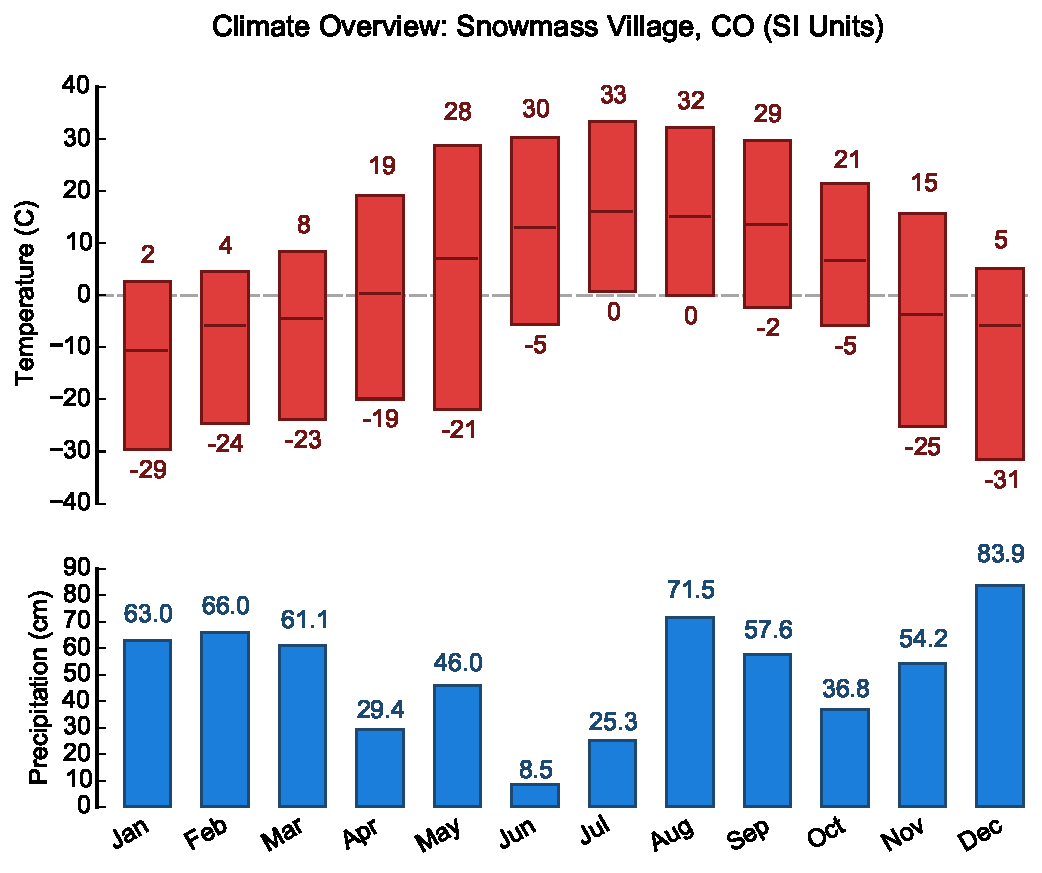
\includegraphics[width=0.9\linewidth]{figures/climate-snowmass.pdf}}
    \caption{A climate chart generated using a statistical query.}
    \label{fig:climate}
\end{figure}

Our second visualization issued queries to retrieve cloud cover information for the entirety of North America. To reduce processing load on the client side, we specified minimum visibility thresholds to eliminate data points that would not be visible in the final output figure. After retrieving this information, we executed a second query that located all areas that exhibited high correlations between cloud cover and precipitation. Figure~\ref{fig:global-contour} illustrates the results of this process for data in July of 2014; cloud cover is represented by white contours with varying opacity, while blue contours describe the correlation between cloud cover and precipitation (darker blues, such as those seen in the top-center of the globe, represent a stronger correlation). Due to the large scope of this visualization (retrieving all data points for a given month across all spatial regions), retrieval took approximately 2.82 seconds, with graphics rendering consuming an additional 1.51 seconds at the client application.

\begin{figure}[b]
    \centerline{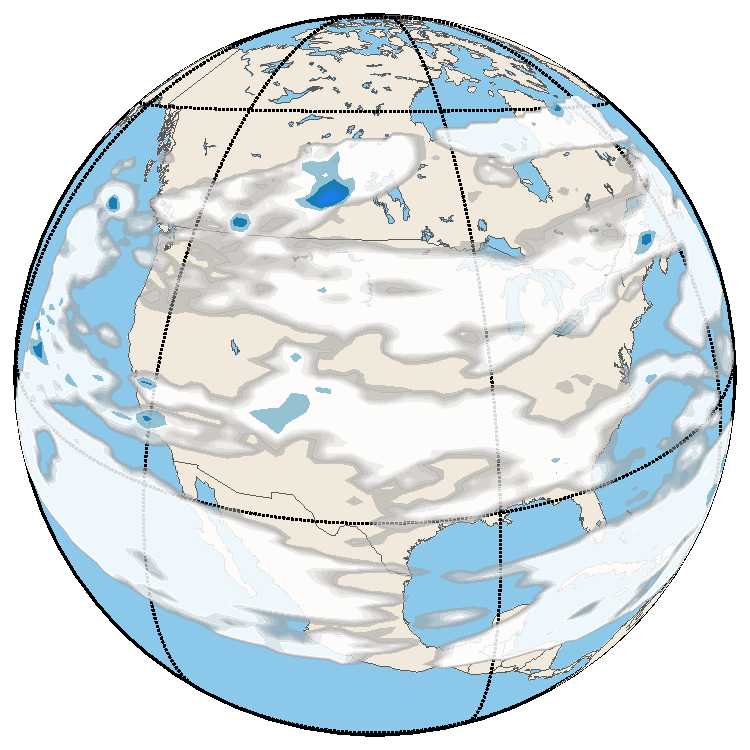
\includegraphics[width=2.5in]{figures/globe.pdf}}
    \caption{Global contour visualization showing cloud cover (white contours) and the correlation with precipitation (blue contours) in July of 2014 across North America.}
    \label{fig:global-contour}
\end{figure}
